\documentclass[12pt,a4paper]{article}
\usepackage[utf8]{inputenc} % For UTF-8 encoding
\usepackage[T1]{fontenc} % For T1 font encoding
\usepackage{graphicx} % For including images
\usepackage{geometry} % For setting page margins
\usepackage{setspace} % For setting line spacing
\usepackage{booktabs} % For better table formatting
\usepackage{multirow} % For multi-row cells in tables
\usepackage{hyperref} % For hyperlinks
\usepackage{float}    % already used for precise float control
\usepackage{placeins} % add this line to enforce float barriers
\usepackage{listings} % For code listings
\usepackage{xcolor} % For colored text

\lstset{
  basicstyle=\ttfamily\small,
  breaklines=true,
  commentstyle=\color{green!50!black},
  keywordstyle=\color{blue},
  stringstyle=\color{red},
  numbers=left,
  numberstyle=\tiny\color{gray},
  numbersep=5pt,
  frame=single,
  framesep=5pt
}

\geometry{
    top=1.5cm,
    bottom=1.5cm,
    left=1.5cm,
    right=1.5cm
}

\begin{document}
\begin{titlepage}
    \begin{minipage}{0.15\textwidth}
        
\includegraphics[width=\linewidth]{Logo/university-logo.png}
    \end{minipage}
    \begin{minipage}{0.625\textwidth}
        \centering
        \MakeUppercase{
            Université Abdelhamidhri Constantine 2\\
            Faculté des Nouvelles Technologies de l'Information et de la Communication NTIC\\
            Le Département Technologies des Logiciels et des Systèmes d'Information TLSI
        }
    \end{minipage}
    \begin{minipage}{0.15\textwidth}
        
\includegraphics[width=\linewidth]{Logo/ntic-logo.png}
    \end{minipage}
    
    \vspace{3cm}

    \begin{center}
        \LARGE{\textbf{TP MEL \\ rapport 3}}
    \end{center}

    \vspace{0.1cm}

    \begin{center}
        SPECIALTY: SOFTWARE ENGINEERING
    \end{center}
    
    \vspace{1.9cm}
    \hrule
    \vspace{0.5cm}

    \begin{center}
        \LARGE{\textbf{Maintenance of Hotel Project (overView)}}
    \end{center}
    
    \vspace{0.5cm}
    \hrule
    \vspace{2cm}
    
    \begin{minipage}[t]{0.66\textwidth}
        \textbf{Supervised by:}\\
        • Dr. Manel DJENOUHAT
    \end{minipage}
    \hfill
    \begin{minipage}[t]{0.4\textwidth}
        \textbf{Presented by:}\\
        • Rouissa Rabah G2\\
        • Belmokhi Dibadj G2\\
        • Brahmia Mohamed\\Haythem Abderrahmen G2
    \end{minipage}

    \vspace{5cm}

    \begin{center}
        \large\textbf{DATE: 14/04/2025}
    \end{center}
\end{titlepage}

\thispagestyle{empty}
\tableofcontents
\newpage
\thispagestyle{empty}
\listoftables
\newpage
\thispagestyle{empty}
\listoffigures
\newpage
\pagenumbering{arabic}

\section{Introduction}
\subsection{Project Context}
The Hotel Management Desktop Application is designed to provide an efficient and reliable solution for managing hotel operations. 
It offers features for handling bookings, managing customer data, tracking reservations, and processing check-ins and check-outs.
The application prioritizes user experience with a clean, intuitive interface.Built with multi-threading capabilities, 
it ensures responsive performance even during peak usage. Comprehensive error handling is integrated throughout to maintain 
stability and prevent data loss or system crashes.

\subsection{Maintenance Objectives}
Ongoing maintenance of the Hotel Management Application focuses on the following key areas:

\subsubsection{Improving Code Readability}
The codebase will be reviewed to ensure that logic is clear and variable names are meaningful. 
Consistent naming practices and well-structured code will help future developers understand and work with the project 
more effectively.

\subsubsection{Removing Code Redundancy}
All duplicate code blocks will be identified and refactored to reduce repetition. This will simplify maintenance, 
lower the risk of bugs, and improve overall code organization.

\subsubsection{Enhancing Code Efficiency}
Unnecessary or overly complex lines of code will be optimized or removed. Where possible, functions and components will be 
simplified into more modular forms, making the system easier to update, extend, and debug.
\subsection{Tools and Methodology}
To ensure the ongoing quality and maintainability of the Hotel Management Application, 
the following tools and practices will be adopted:

\subsubsection{SonarCloud}
SonarCloud will be used to perform regular static code analysis. It will help in detecting code smells, potential bugs, 
and overly complex code structures. By addressing these issues promptly, the codebase will remain clean, maintainable, 
and easier for future developers to work with.
\subsubsection{GitHub}
Version control will be handled through GitHub, providing a centralized platform for tracking changes, managing branches, 
and collaborating on updates. This ensures that all development activity is traceable and well-documented, reducing the 
risk of conflicts or data loss.By continuously improving code quality and keeping the system free from unnecessary complexity, 
the Hotel Management Application will remain robust, easy to maintain, and efficient, without compromising its core features.

\section{Analysis of Current State}
\subsection{SonarQube Metrics Overview}
\begin{figure}[H]
    \centering
    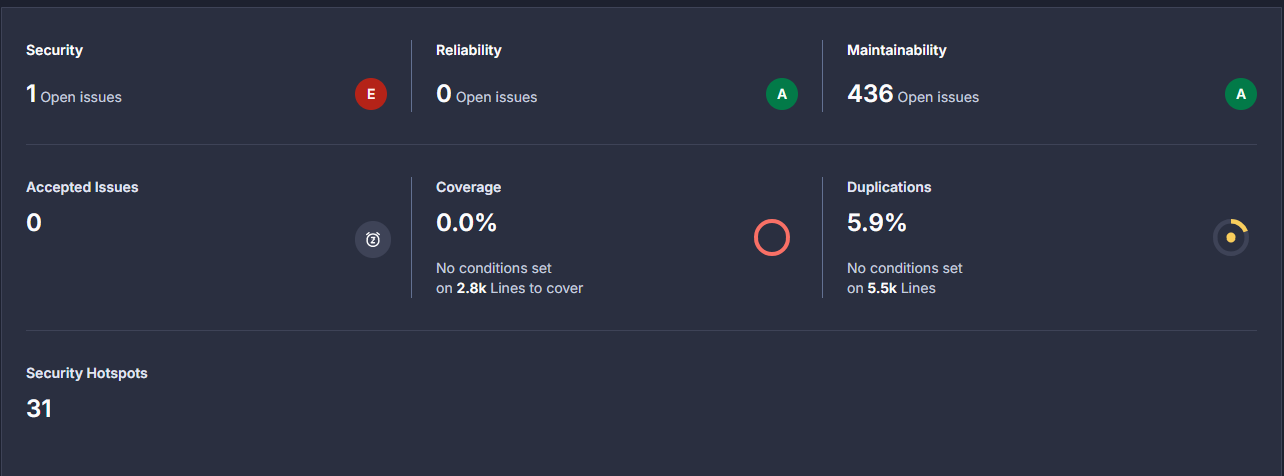
\includegraphics[width=1\textwidth]{AbdouPhotos/Maintainability/SummaryBefore.png}
    \caption{SonarQube Metrics Overviewe}
    \label{fig:SMO}
\end{figure}

\section{Identified Issues}
\subsection{Security Issues}
\begin{figure}[H]
    \centering
    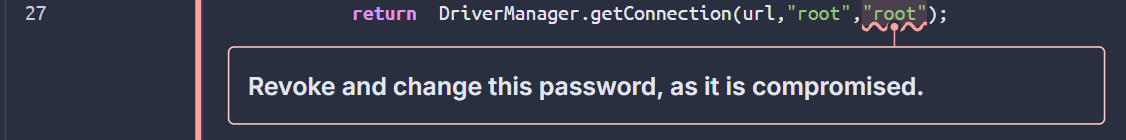
\includegraphics[width=1\textwidth]{AbdouPhotos/Security/SecurityIssue.png}
    \caption{Security Issues}
    \label{fig:SI}
\end{figure}
\begin{figure}[H]
    \centering
    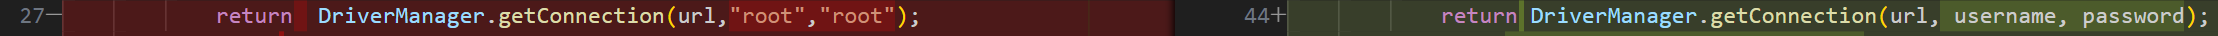
\includegraphics[width=1\textwidth]{AbdouPhotos/Security/SecurityIssueSolution.png}
    \caption{ Security Issue -  Issue Solution}
    \label{fig:MI-1stS}
\end{figure}

\subsection{Maintinability Issues}
\begin{figure}[H]
    \centering
    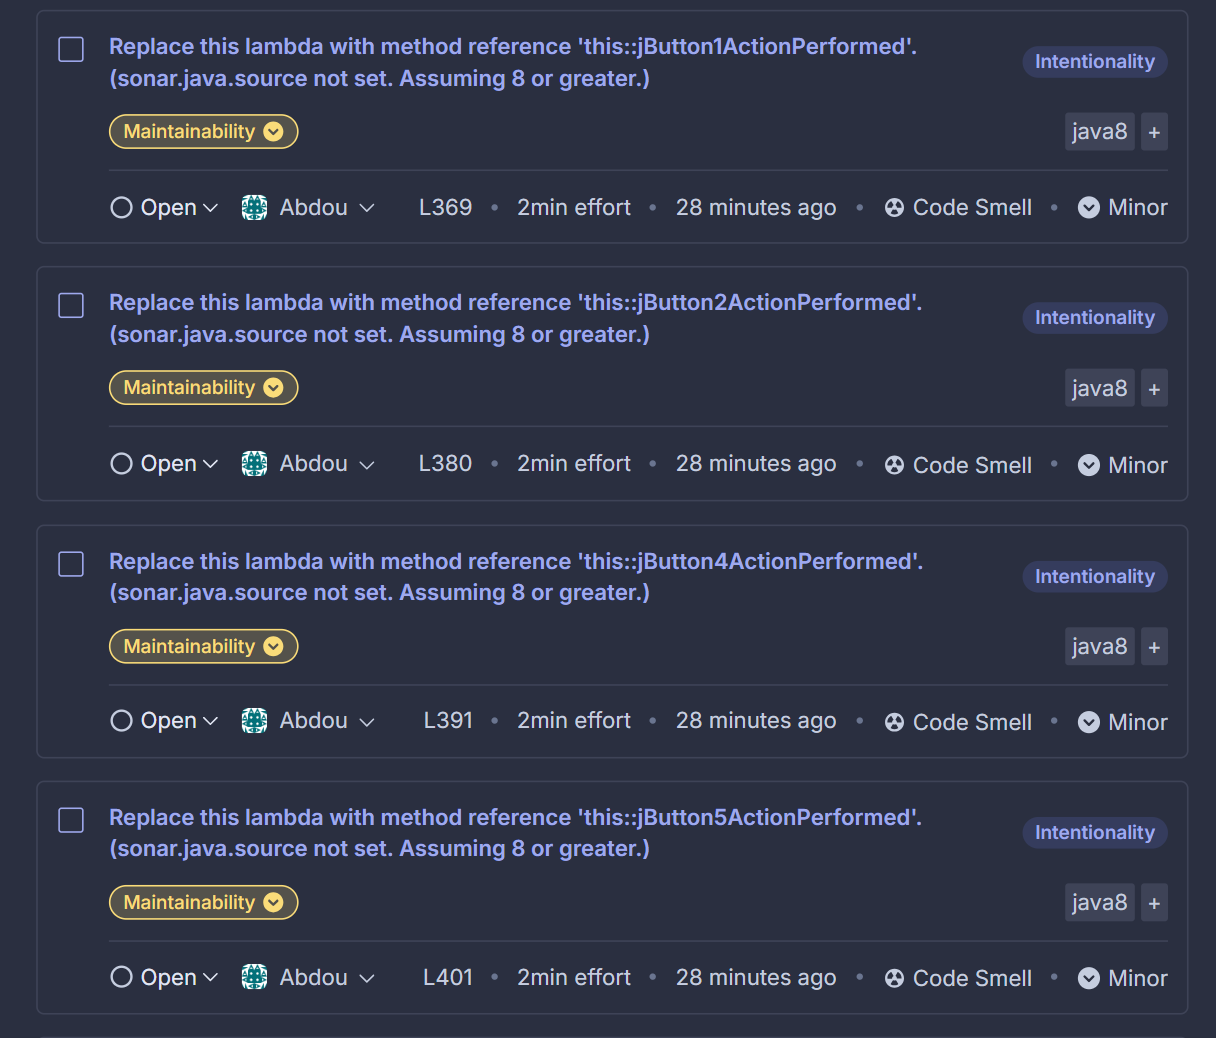
\includegraphics[width=0.8\textwidth]{AbdouPhotos/Maintainability/MaintainabilityOverview.png}
    \caption{Maintainability Issues Overview}
    \label{fig:40I}
\end{figure}
\begin{figure}[H]
    \centering
    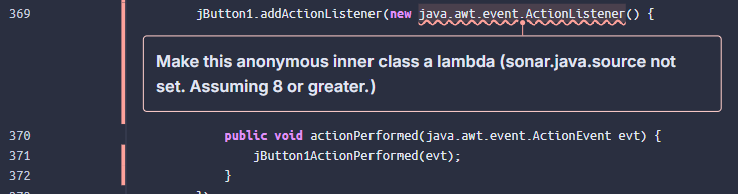
\includegraphics[width=1\textwidth]{AbdouPhotos/Maintainability/jButton1.png}
    \caption{Maintainability Issues - First Issue}
    \label{fig:MI-1st}
\end{figure}
\begin{figure}[H]
    \centering
    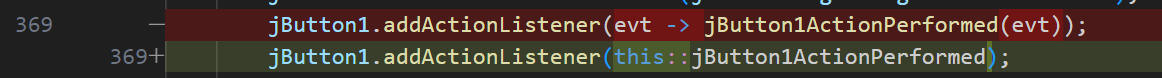
\includegraphics[width=1\textwidth]{AbdouPhotos/Maintainability/jButton1Solution.png}
    \caption{Maintainability Issues - First Issue Solution}
    \label{fig:MI-1stS}
\end{figure}
\begin{figure}[H]
    \centering
    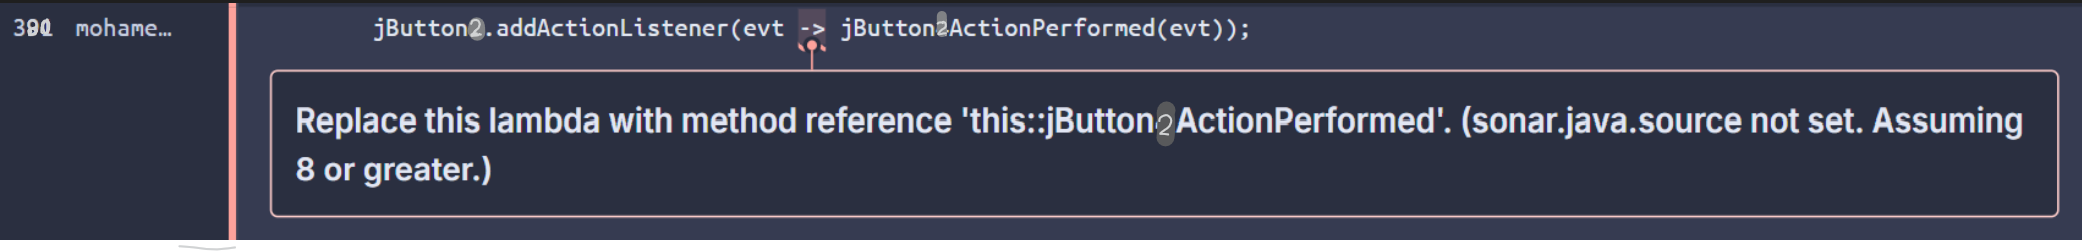
\includegraphics[width=1\textwidth]{AbdouPhotos/Maintainability/jButton2.png}
    \caption{Maintainability Issues - Second Issue}
    \label{fig:MI-2nd}
\end{figure}
\begin{figure}[H]
    \centering
    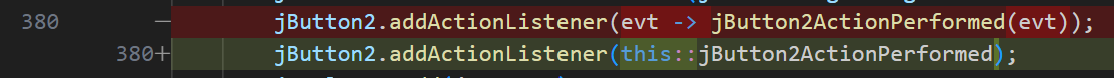
\includegraphics[width=1\textwidth]{AbdouPhotos/Maintainability/jButton2Solution.png}
    \caption{Maintainability Issues - Second Issue Solution}
    \label{fig:MI-2ndS}
\end{figure}
\begin{figure}[H]
    \centering
    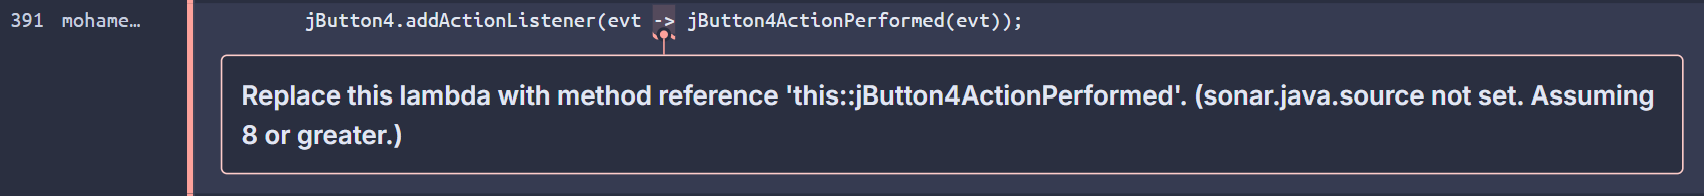
\includegraphics[width=1\textwidth]{AbdouPhotos/Maintainability/jButton4.png}
    \caption{Maintainability Issues - Fourth Issue}
    \label{fig:MI-4th}
\end{figure}
\begin{figure}[H]
    \centering
    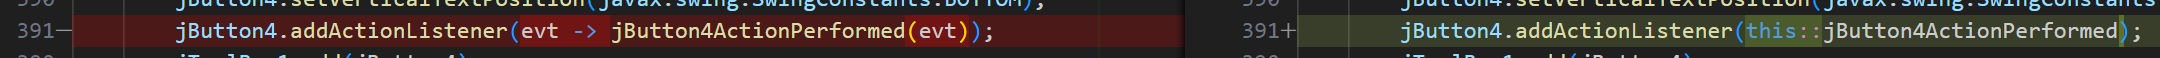
\includegraphics[width=1\textwidth]{AbdouPhotos/Maintainability/jButton4Solution.png}
    \caption{Maintainability Issues - Fourth Issue Solution}
    \label{fig:MI-4thS}
\end{figure}
\begin{figure}[H]
    \centering
    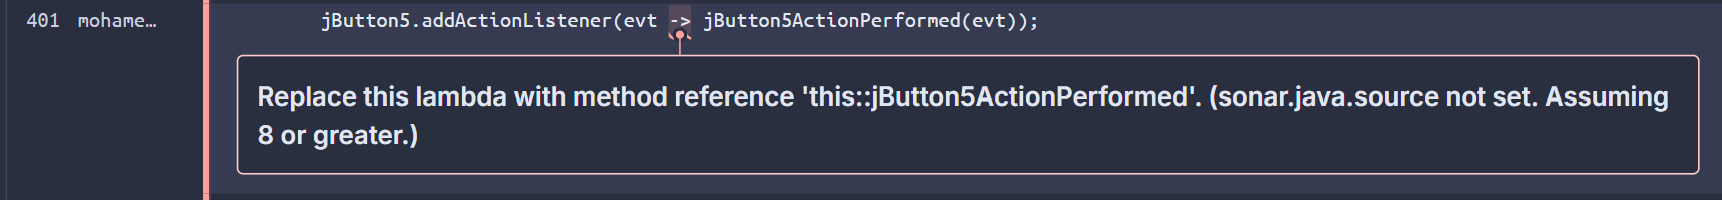
\includegraphics[width=1\textwidth]{AbdouPhotos/Maintainability/jButton5.png}
    \caption{Maintainability Issues - Fifth Issue}
    \label{fig:MI-5th}
\end{figure}
\begin{figure}[H]
    \centering
    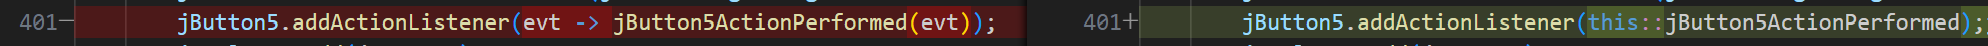
\includegraphics[width=1\textwidth]{AbdouPhotos/Maintainability/jButton5Solution.png}
    \caption{Maintainability Issues - Fifth Issue Solution}
    \label{fig:MI-5thS}
\end{figure}
\begin{figure}[H]
    \centering
    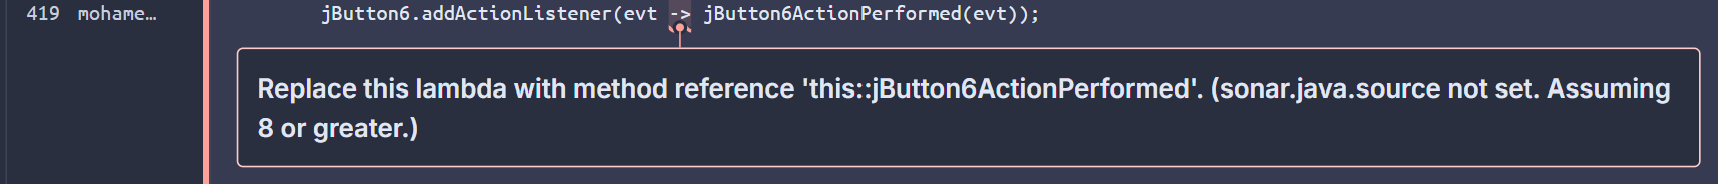
\includegraphics[width=1\textwidth]{AbdouPhotos/Maintainability/jButton6.png}
    \caption{Maintainability Issues - Sixth Issue}
    \label{fig:MI-6th}
\end{figure}
\begin{figure}[H]
    \centering
    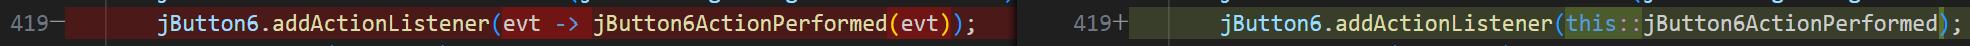
\includegraphics[width=1\textwidth]{AbdouPhotos/Maintainability/jButton6Solution.png}
    \caption{Maintainability Issues - Sixth Issue Solution}
    \label{fig:MI-6thS}
\end{figure}
\begin{figure}[H]
    \centering
    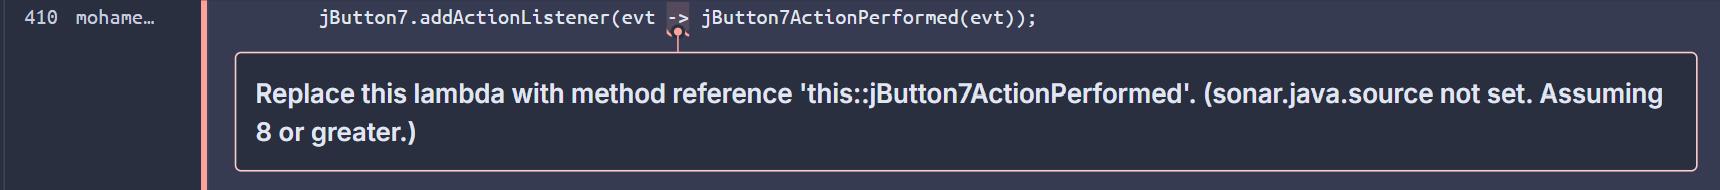
\includegraphics[width=1\textwidth]{AbdouPhotos/Maintainability/jButton7.png}
    \caption{Maintainability Issues - Seventh Issue}
    \label{fig:MI-7th}
\end{figure}
\begin{figure}[H]
    \centering
    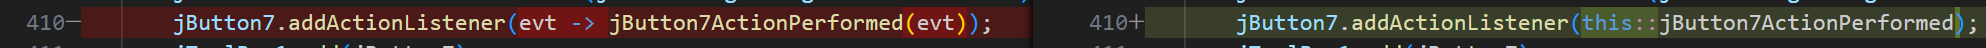
\includegraphics[width=1\textwidth]{AbdouPhotos/Maintainability/jButton7Solution.png}
    \caption{Maintainability Issues - Seventh Issue Solution}
    \label{fig:MI-7thS}
\end{figure}
\section{Results and Verification}
\subsection{SonarQube Results After Maintenance}

\begin{figure}[H]
    \centering
    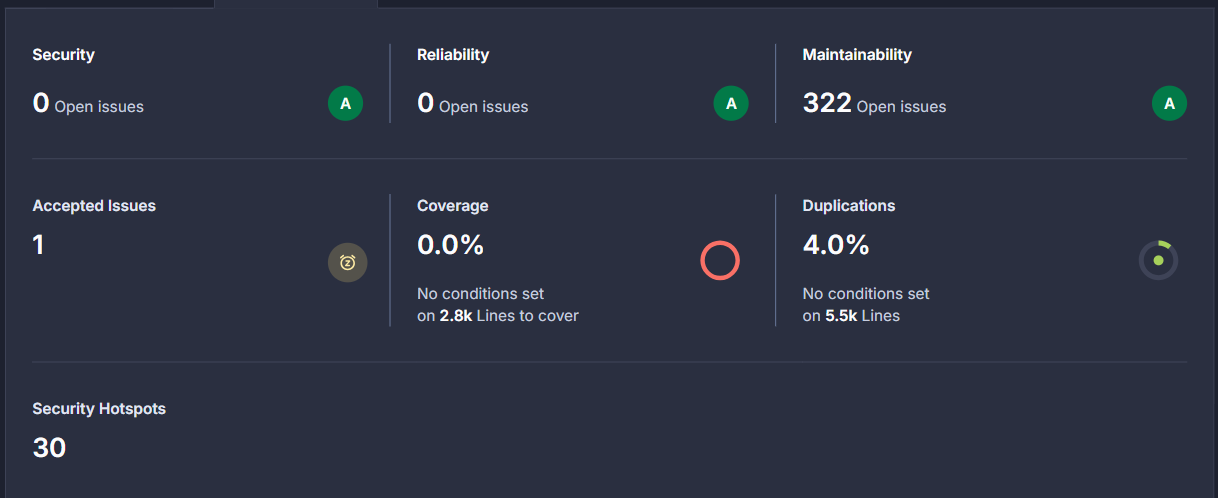
\includegraphics[width=1\textwidth]{AbdouPhotos/Maintainability/ResultAfter.png}
    \caption{SonarQube Metrics Overview After Maintenance}
    \label{fig:SMO-A}
\end{figure}

\begin{table}[H]
\centering
\begin{tabular}{lcc}
\toprule
\textbf{Metric} & \textbf{Before} & \textbf{After} \\ 
\midrule
Security Issues & 1 & 0 \\ 
Reliability Issues & 0 & 0 \\ 
Maintainability Issues & 436 & 322 \\ 
Accepted Issues & 0 & 1 \\ 
Coverage & Not configured & Not configured \\ 
Duplications & 5.9\% & 4.0\% \\ 
Security Hotspots & 31 & 30 \\ 
\bottomrule
\end{tabular}
\caption{SonarQube Analysis Results - Before vs. After}
\end{table}

\end{document}

